\chapter{Resultados y Análisis Exploratorio}

Esta sección se apoya en \texttt{outputs/analisis\_exploratorio.md}, \texttt{outputs/tablas\_hallazgos\_fase9.csv}, los rankings exportados y las figuras generadas en Fase 9. La lectura se mantiene en un plano estrictamente descriptivo.

\section{Rankings por dimensión}

Los menores valores observados de \texttt{areas\_verdes\_m2\_hab} corresponden a CONCHALI, CERRILLOS, INDEPENDENCIA, LA CISTERNA, SAN MIGUEL. En pobreza por ingresos, los mayores valores observados corresponden a LA PINTANA, SAN RAMON, LO ESPEJO, EL BOSQUE, CONCHALI. En \texttt{ipp\_pesos\_hab}, los menores valores observados corresponden a CERRO NAVIA, LA PINTANA, LO PRADO, EL BOSQUE, LA GRANJA.

\begin{table}[htbp]
\centering
\footnotesize
\caption{Resumen de hallazgos descriptivos reutilizables desde los outputs de Fase 9.}
\begin{tabular}{|p{4.3cm}|p{7.0cm}|p{3.0cm}|}
\hline
Hallazgo & Comunas observadas & Output fuente \\
\hline
Menor áreas verdes por habitante & CONCHALI, CERRILLOS, INDEPENDENCIA, LA CISTERNA, SAN MIGUEL & outputs/ranking\_areas\_verdes.csv \\
Mayor pobreza por ingresos & LA PINTANA, SAN RAMON, LO ESPEJO, EL BOSQUE, CONCHALI & outputs/ranking\_pobreza.csv \\
Menor IPP por habitante & CERRO NAVIA, LA PINTANA, LO PRADO, EL BOSQUE, LA GRANJA & outputs/ranking\_ipp.csv \\
Peor quintil simultáneo de pobreza y áreas verdes & CONCHALI & outputs/tablas\_hallazgos\_fase9.csv \\
Peor quintil simultáneo de pobreza e IPP & LA PINTANA, SAN RAMON, LO ESPEJO, EL BOSQUE, LA GRANJA, CERRO NAVIA & outputs/tablas\_hallazgos\_fase9.csv \\
Rezago crítico en al menos dos dimensiones & LO ESPEJO, EL BOSQUE, CONCHALI, LA PINTANA, SAN RAMON, LA GRANJA, CERRO NAVIA & outputs/indice\_rezago\_territorial.csv \\
\hline
\end{tabular}
\end{table}


\begin{figure}[htbp]
\centering
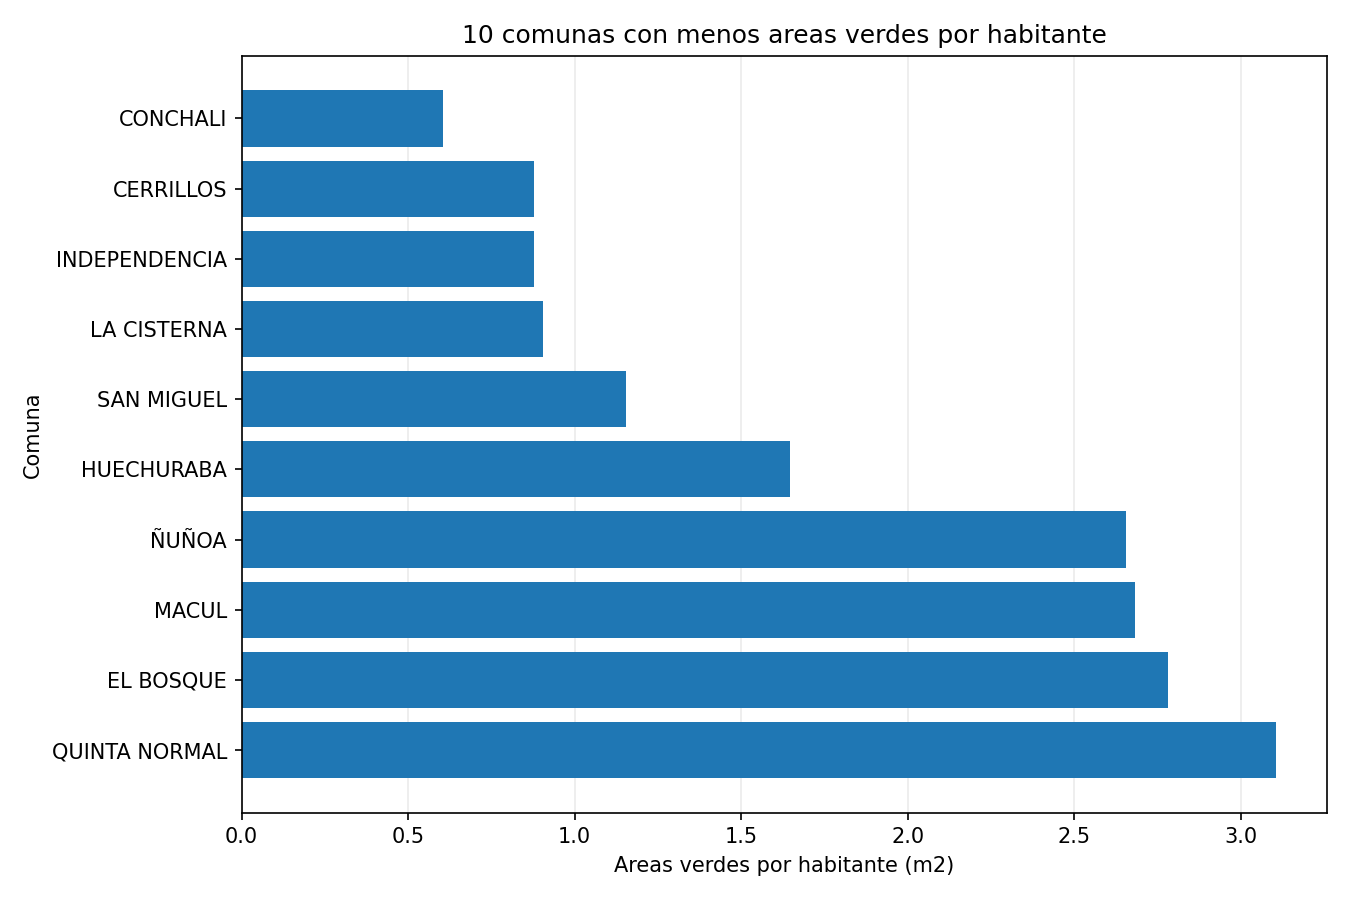
\includegraphics[width=0.88\textwidth]{Figuras/areas_verdes_m2_hab_bottom10.png}
\caption{Diez comunas con menor disponibilidad de áreas verdes por habitante.}
\end{figure}

\begin{figure}[htbp]
\centering
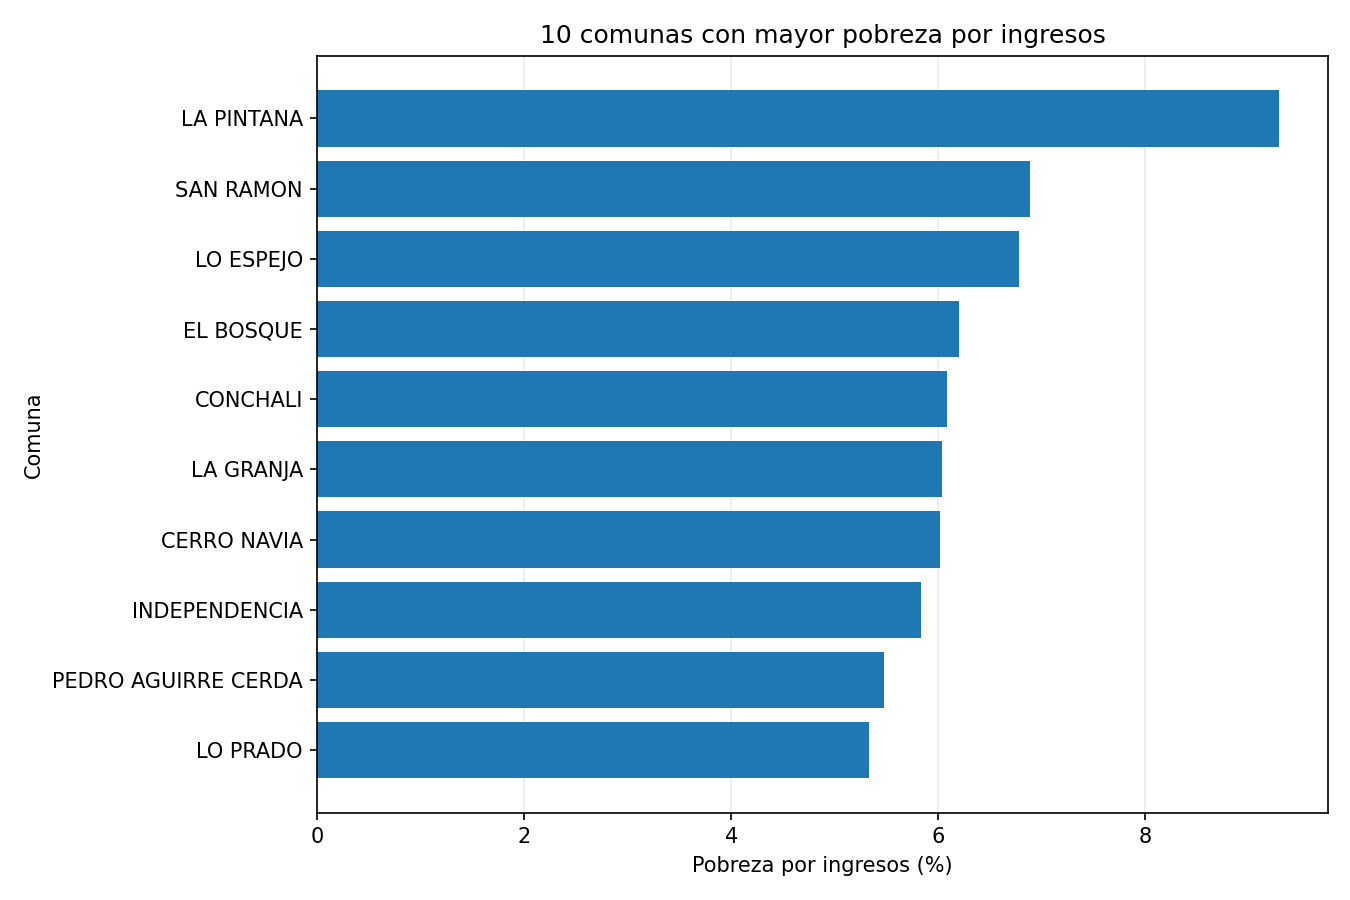
\includegraphics[width=0.88\textwidth]{Figuras/pobreza_ingresos_top10.png}
\caption{Diez comunas con mayor pobreza por ingresos en el dataset final.}
\end{figure}

\begin{figure}[htbp]
\centering
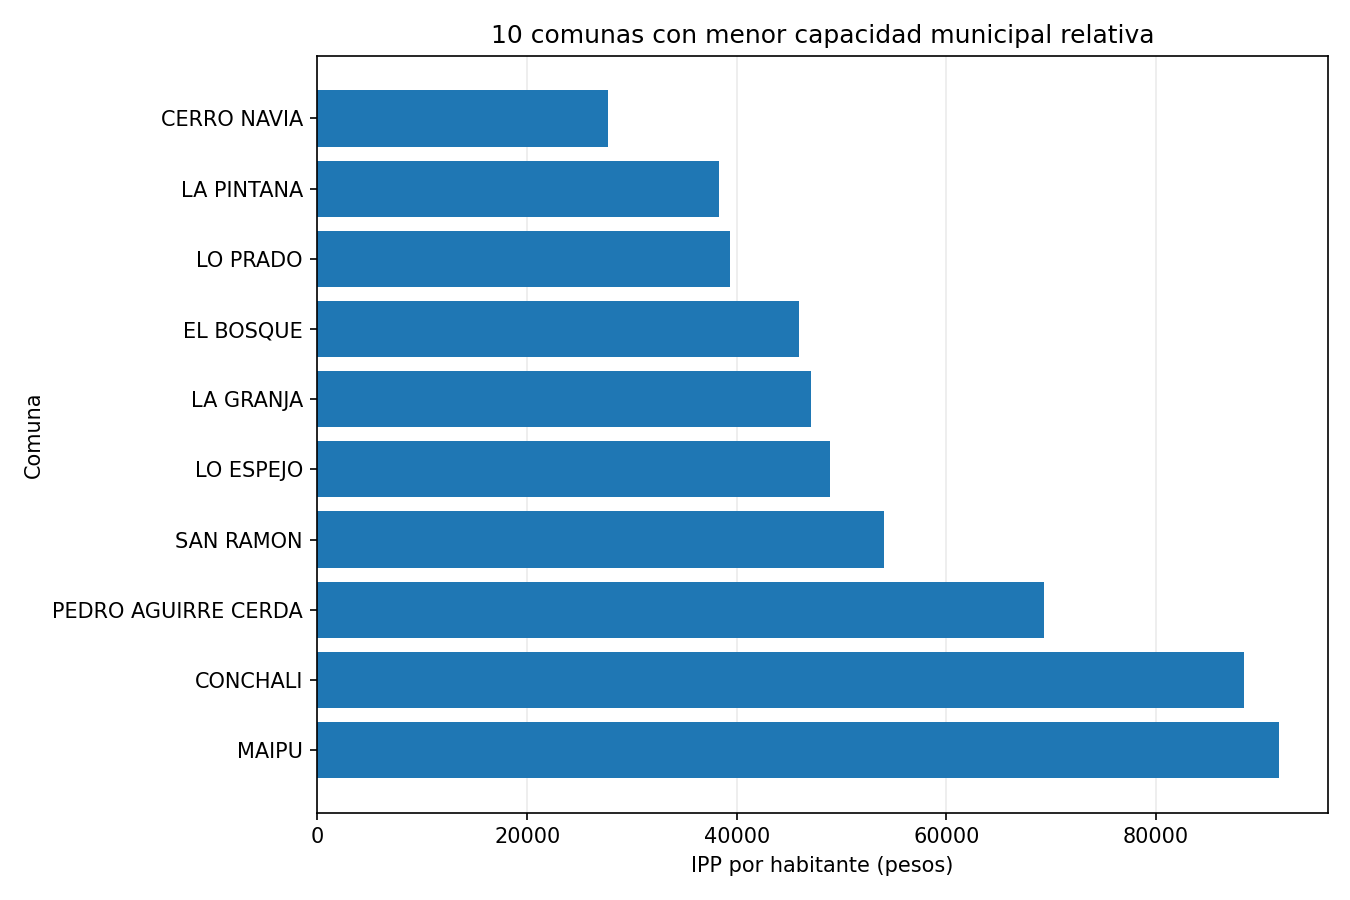
\includegraphics[width=0.88\textwidth]{Figuras/ipp_pesos_hab_bottom10.png}
\caption{Diez comunas con menor IPP por habitante en el dataset final.}
\end{figure}

\section{Cruces descriptivos y rezago en múltiples dimensiones}

El cruce por quintiles muestra que el peor quintil simultáneo de pobreza y áreas verdes por habitante se observa en CONCHALI. Por su parte, el peor quintil simultáneo de pobreza e IPP por habitante se observa en LA PINTANA, SAN RAMON, LO ESPEJO, EL BOSQUE, LA GRANJA, CERRO NAVIA. Al ampliar la mirada a rezago crítico en al menos dos dimensiones, aparecen LO ESPEJO, EL BOSQUE, CONCHALI, LA PINTANA, SAN RAMON, LA GRANJA, CERRO NAVIA.

El índice auxiliar de rezago territorial, definido en Fase 9 como suma de quintiles de rezago, ordena en los primeros lugares a Conchalí, El Bosque, Lo Espejo, La Pintana y San Ramón. Este índice se interpreta solo como apoyo descriptivo para resumir coincidencias de rezago relativo entre comunas.

\begin{table}[htbp]
\centering
\scriptsize
\caption{Comunas con rezago crítico en al menos dos dimensiones del análisis auxiliar.}
\begin{tabular}{|c|p{3.0cm}|p{1.6cm}|p{2.0cm}|p{2.2cm}|c|c|}
\hline
Código & Comuna & Pobreza & Áreas/hab & IPP/hab & Dim. & Índice \\
\hline
13116 & LO ESPEJO & 6.7817 & 3.344647 & 48908.769116 & 2 & 14 \\
13105 & EL BOSQUE & 6.1982 & 2.780551 & 45941.619379 & 2 & 14 \\
13104 & CONCHALI & 6.0799 & 0.603247 & 88427.175603 & 2 & 14 \\
13112 & LA PINTANA & 9.2938 & 4.309741 & 38281.739358 & 2 & 13 \\
13131 & SAN RAMON & 6.8821 & 5.256743 & 54032.104418 & 2 & 13 \\
13111 & LA GRANJA & 6.0302 & 6.233793 & 47063.353627 & 2 & 12 \\
13103 & CERRO NAVIA & 6.0135 & 5.851764 & 27701.980354 & 2 & 12 \\
\hline
\end{tabular}
\end{table}


\begin{figure}[htbp]
\centering
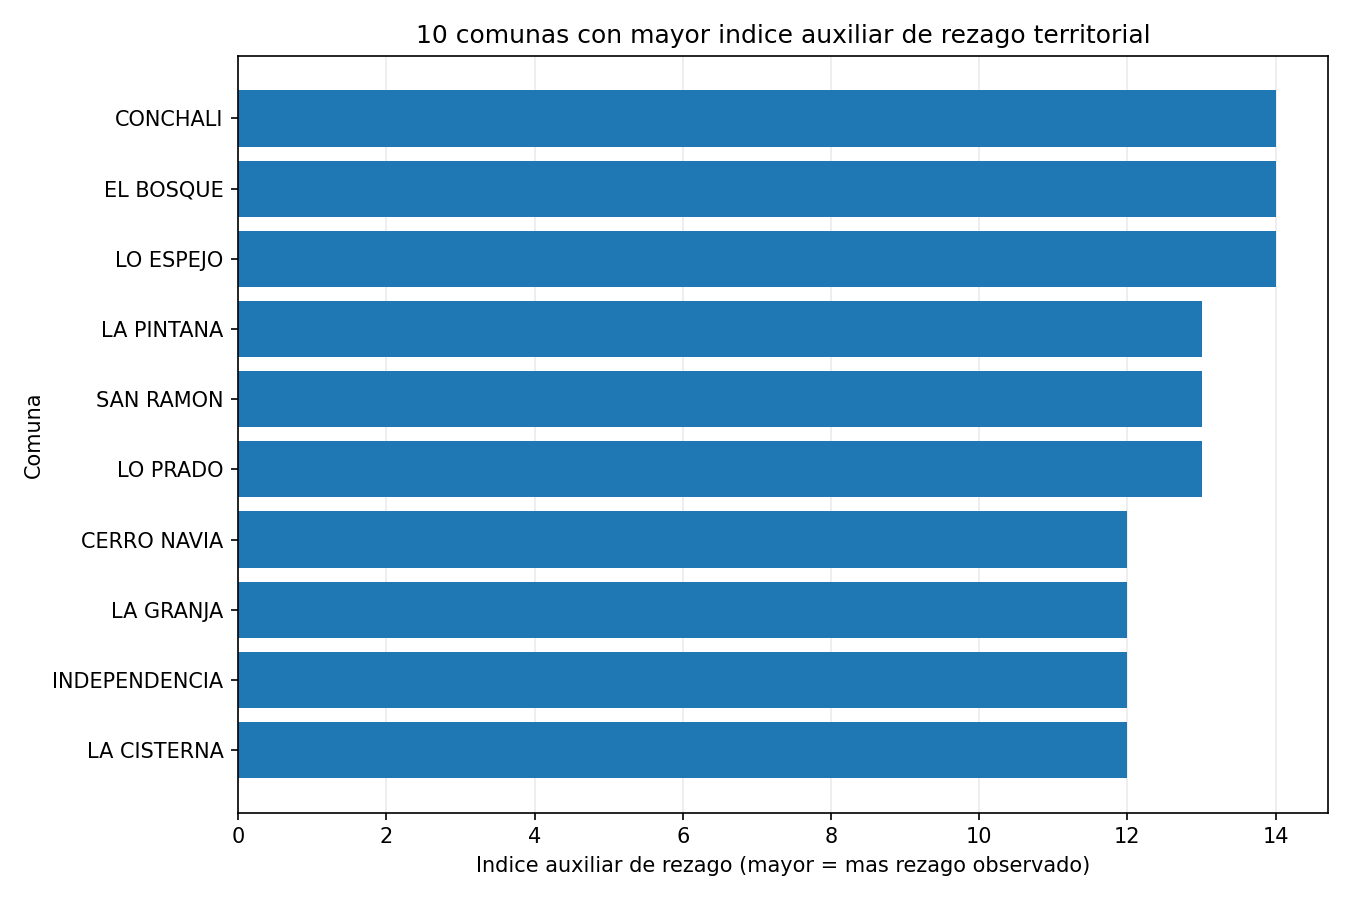
\includegraphics[width=0.88\textwidth]{Figuras/indice_rezago_territorial_top10.png}
\caption{Diez comunas con mayor índice auxiliar de rezago territorial.}
\end{figure}

\section{Lectura descriptiva del scatter y tratamiento del outlier}

El scatter de pobreza y áreas verdes por habitante se mantiene como evidencia exploratoria y no como prueba de relación causal. Su lectura exige una advertencia metodológica explícita: Quilicura registra \texttt{areas\_verdes\_m2\_hab = 3931.614773}, muy por encima de La Reina (21.734172) y Providencia (20.172865). Por esta razón, el gráfico fue documentado con escala logarítmica en el eje X para preservar visibilidad sobre el resto de las comunas.

\begin{figure}[htbp]
\centering
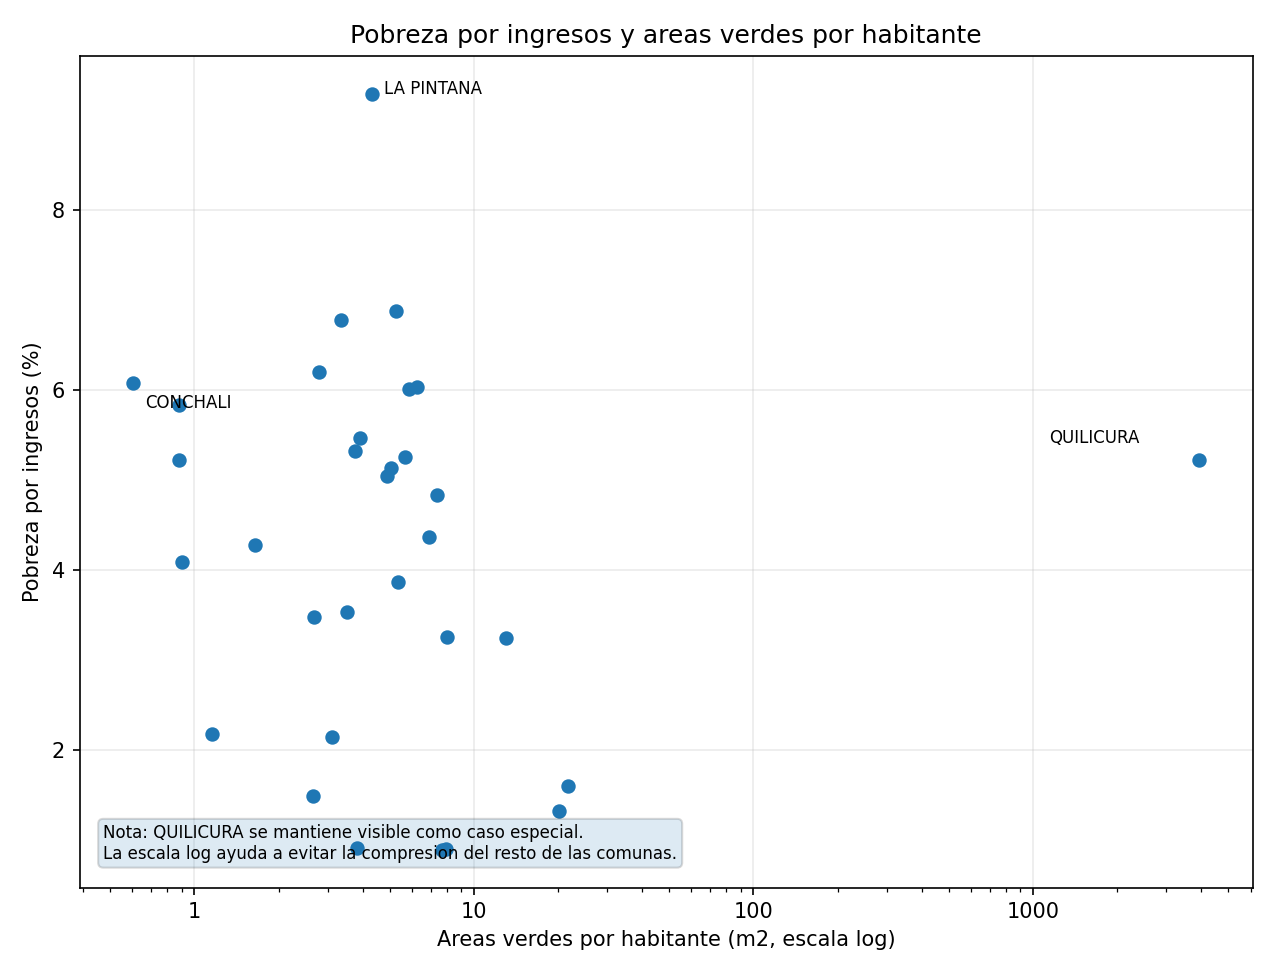
\includegraphics[width=0.88\textwidth]{Figuras/pobreza_vs_areas_verdes_scatter.png}
\caption{Scatter descriptivo entre pobreza por ingresos y áreas verdes por habitante.}
\end{figure}

En términos comunicacionales, el caso de Quilicura debe tratarse como outlier plausible y no como valor descartado. El repositorio no aporta evidencia para clasificarlo como error; por lo tanto, la decisión metodológica correcta es mantenerlo, advertir su influencia en la escala y evitar interpretaciones causales a partir del gráfico.
